\begin{frame}{Metric Learning: From Labels to Distances}
  \begin{columns}[T,onlytextwidth]
    \column{0.56\textwidth}
      \begin{itemize}\footnotesize\itemsep0.35em
        \item \textbf{Goal:} learn an embedding $f:\mathcal{X}\to\mathbb{R}^d$ with $\lVert f(x)\rVert_2=1$, so that the distance $d(x,x')=\lVert f(x)-f(x')\rVert_2$ is small for two images of the same class and large otherwise. For unit vectors $d^2=2-2\cos\big(f(x),f(x')\big)$, so distance and cosine similarity rank neighbours identically.
        \item \textbf{Why not a softmax head:} it has one output per training class and cannot name a class it never saw. Retrieval, face verification (same person or not) and re-identification meet new classes at test time, so they compare embeddings by $k$-NN search or with a distance threshold.
        \item \textbf{Zero-shot split:} train on the first half of the classes, test on the disjoint second half. CUB-200-2011: 100 + 100 species; Cars196 (Stanford Cars): 98 + 98 models; Stanford Online Products (SOP): 120{,}053 eBay images of 11{,}318 + 11{,}316 products.
      \end{itemize}
    \column{0.42\textwidth}
      \centering
      \vspace{0.2em}
      \begin{tikzpicture}[font=\sffamily\scriptsize, >=latex,
          ca/.style={circle, fill=blue!60, inner sep=1.5pt},
          cb/.style={circle, fill=orange!85, inner sep=1.5pt},
          cc/.style={circle, fill=green!50!black, inner sep=1.5pt}]
        \draw[gray!60, thick] (0,0) circle (1.3);
        \fill[gray!70!black] (0,0) circle (0.9pt);
        \foreach \a in {10,20,34,48,56} {\node[ca] at (\a:1.3) {};}
        \foreach \a in {128,140,151,163,172} {\node[cb] at (\a:1.3) {};}
        \foreach \a in {232,246,258,270,284} {\node[cc] at (\a:1.3) {};}
        \draw[->, gray!70!black] (0,0) -- (163:1.22) node[pos=0.5, sloped, above] {$f(x)$};
        % query at 41 deg: its 3 nearest points are at 34, 48 and 56 deg; the next one (20 deg) is outside the arc
        \node[star, star points=5, star point ratio=2.2, fill=blue!60, draw=red, thick, inner sep=1.2pt] at (41:1.3) {};
        \node at (41:1.02) {$q$};
        \draw[red!80!black, thick] (29:1.56) arc[start angle=29, end angle=61, radius=1.56];
        \node[red!80!black, anchor=south west, align=left] at (45:1.6) {$K=3$ nearest\\neighbours of $q$};
      \end{tikzpicture}\\[0.3em]
      {\scriptsize Unit-norm embeddings lie on a sphere; colours are classes. The query $q$ (star, red outline) retrieves its $K=3$ nearest neighbours, all of its own class.\par}
      \vspace{0.5em}
      {\scriptsize Split: Song et al., ``Deep Metric Learning via Lifted Structured Feature Embedding,'' CVPR 2016, \href{https://openaccess.thecvf.com/content_cvpr_2016/papers/Song_Deep_Metric_Learning_CVPR_2016_paper.pdf}{OpenAccess}, Sec.~7.\par}
  \end{columns}
\end{frame}

\begin{frame}{Ranking Metrics: Recall@K and MAP@R}
  \begin{columns}[T,onlytextwidth]
    \column{0.54\textwidth}
      \begin{itemize}\footnotesize\itemsep0.35em
        \item \textbf{Recall@$K$:} each test image queries the rest of the test set and scores 1 if an image of its class is among its $K$ nearest neighbours:
        \[ \text{Recall@}K=\frac{1}{|Q|}\sum_{q\in Q}\mathbf{1}\big[\,\exists\, j\in\mathcal{N}_K(q):\ y_j=y_q\,\big] \]
        $Q$: the test queries; $\mathcal{N}_K(q)$: the $K$ test images nearest to $q$, excluding $q$; $y$: class label; $\mathbf{1}[\cdot]$: 1 if the condition holds, else 0.
        \item \textbf{MAP@$R$} (mean average precision at $R$): for a query with $R$ same-class images in the test set, look at its $R$ nearest neighbours:
        \[ \text{MAP@}R=\frac{1}{R}\sum_{i=1}^{R}P(i) \]
        $P(i)$: the precision at rank $i$ if result $i$ is correct, else 0; averaged over queries.
      \end{itemize}
    \column{0.44\textwidth}
      \centering
      \vspace{0.6em}
      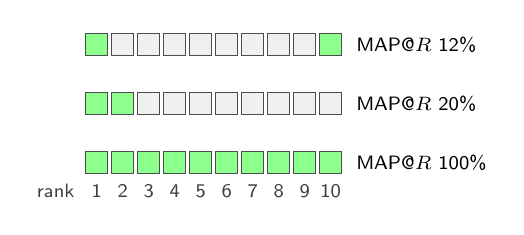
\begin{tikzpicture}[font=\sffamily\scriptsize]
        \foreach \col [count=\pos] in {green!45,gray!12,gray!12,gray!12,gray!12,gray!12,gray!12,gray!12,gray!12,green!45}
          \node[draw=gray!60!black, fill=\col, minimum size=0.28cm, inner sep=0pt] at (0.33*\pos,1.5) {};
        \foreach \col [count=\pos] in {green!45,green!45,gray!12,gray!12,gray!12,gray!12,gray!12,gray!12,gray!12,gray!12}
          \node[draw=gray!60!black, fill=\col, minimum size=0.28cm, inner sep=0pt] at (0.33*\pos,0.75) {};
        \foreach \pos in {1,...,10}
          \node[draw=gray!60!black, fill=green!45, minimum size=0.28cm, inner sep=0pt] at (0.33*\pos,0) {};
        \foreach \pos in {1,...,10}
          \node[gray!50!black] at (0.33*\pos,-0.36) {\pos};
        \node[anchor=west] at (3.5,1.5) {MAP@$R$ 12\%};
        \node[anchor=west] at (3.5,0.75) {MAP@$R$ 20\%};
        \node[anchor=west] at (3.5,0) {MAP@$R$ 100\%};
        \node[gray!50!black, anchor=east] at (0.17,-0.36) {rank};
      \end{tikzpicture}\\[0.4em]
      {\scriptsize One query with $R=10$ same-class images; green: correct result. Recall@1 is 100\% in all three rows, yet MAP@$R$ separates them: $(1+2/10)/10=12\%$ in the top row. Recall@$K$: Song et al., CVPR 2016, Sec.~6. After Musgrave et al., ``A Metric Learning Reality Check,'' ECCV 2020, \href{https://arxiv.org/abs/2003.08505v3}{arXiv:2003.08505v3}, Table~3.\par}
      \begin{itemize}\scriptsize\itemsep0.2em
        \item Musgrave et al.\ report MAP@$R$ because it rewards well-clustered embeddings and is steadier during training: lag-one autocorrelation of validation accuracy 0.81, against 0.73 for Recall@1 (Sec.~3.2).
      \end{itemize}
  \end{columns}
\end{frame}

\begin{frame}{Pair and Triplet Losses}
  \begin{columns}[T,onlytextwidth]
    \column{0.52\textwidth}
      \begin{itemize}\footnotesize\itemsep0.35em
        \item \textbf{Contrastive loss} (Hadsell et al., CVPR 2006), a margin-based pair loss distinct from InfoNCE and NT-Xent, on a pair $(x_i,x_j)$ with $y_{ij}=1$ if both images share a class, else 0:
        \[ \mathcal{L}_{\text{con}}=y_{ij}\,\tfrac{1}{2}\,d_{ij}^{2}+(1-y_{ij})\,\tfrac{1}{2}\,\big[m-d_{ij}\big]_+^{2} \]
        $d_{ij}=d(x_i,x_j)$; $[u]_+=\max(0,u)$; the \textbf{margin} $m>0$ is the gap the loss demands: a negative pair farther apart than $m$ adds no loss.
        \item \textbf{Triplet loss} (Schroff et al., FaceNet, CVPR 2015) on an anchor $a$, a positive $p$ (same class) and a negative $n$ (another class):
        \[ \mathcal{L}_{\text{tri}}=\big[\,d(a,p)^2-d(a,n)^2+m\,\big]_+ \]
        summed over triplets. FaceNet used $m=0.2$ on 128-d unit-norm face embeddings.
        \item The triplet loss constrains only relative distances, so a class may spread out as long as other classes stay farther away; the contrastive loss applies one radius to every pair.
      \end{itemize}
    \column{0.46\textwidth}
      \centering
      \vspace{0.4em}
      \resizebox{\linewidth}{!}{%
      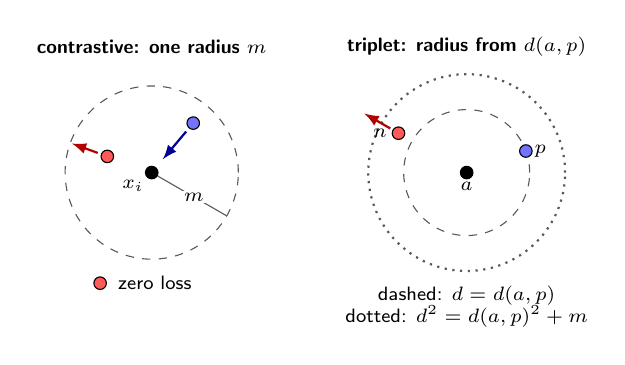
\begin{tikzpicture}[font=\sffamily\scriptsize, >=latex,
          pt/.style={circle, draw=black, inner sep=1.6pt},
          posp/.style={pt, fill=blue!55},
          negp/.style={pt, fill=red!65},
          ancp/.style={pt, fill=black}]
        \node[font=\sffamily\scriptsize\bfseries] at (0,1.6) {contrastive: one radius $m$};
        \draw[dashed, gray!70!black] (0,0) circle (1.1);
        \draw[gray!70!black] (0,0) -- (-30:1.1);
        \node[fill=white, inner sep=0.8pt] at (-30:0.62) {$m$};
        \node[ancp] at (0,0) {};
        \node[anchor=north east, inner sep=1pt] at (-0.06,-0.06) {$x_i$};
        \node[posp] at (50:0.82) {};
        \draw[->, blue!60!black, thick] (50:0.68) -- (50:0.22);
        \node[negp] at (160:0.6) {};
        \draw[->, red!70!black, thick] (160:0.73) -- (160:1.08);
        \node[negp] at (245:1.55) {};
        \node[anchor=west, xshift=3pt] at (245:1.55) {zero loss};
        % triplet panel: dashed radius d(a,p) = 0.8; dotted radius sqrt(0.8^2 + m) = 1.25
        \begin{scope}[xshift=4.0cm]
          \node[font=\sffamily\scriptsize\bfseries] at (0,1.6) {triplet: radius from $d(a,p)$};
          \draw[dashed, gray!70!black] (0,0) circle (0.8);
          \draw[dotted, thick, gray!70!black] (0,0) circle (1.25);
          \node[ancp] at (0,0) {};
          \node[anchor=north, inner sep=1pt] at (0,-0.08) {$a$};
          \node[posp] at (20:0.8) {};
          \node[anchor=west, inner sep=1pt, xshift=2pt] at (20:0.8) {$p$};
          \node[negp] at (150:1.0) {};
          \node[anchor=east, inner sep=1pt, xshift=-3pt] at (150:1.0) {$n$};
          \draw[->, red!70!black, thick] (150:1.12) -- (150:1.5);
          \node[anchor=north, align=center] at (0,-1.32) {dashed: $d=d(a,p)$\\dotted: $d^2=d(a,p)^2+m$};
        \end{scope}
      \end{tikzpicture}}\\[0.3em]
      {\scriptsize Black: anchor; blue: same class; red: other class. Left: same-class points are pulled in and other classes pushed out to radius $m$. Right: the triplet margin is measured from the positive's distance.\par}
      \vspace{0.5em}
      {\scriptsize Hadsell et al., ``Dimensionality Reduction by Learning an Invariant Mapping,'' CVPR 2006, \href{https://doi.org/10.1109/CVPR.2006.100}{doi:10.1109/CVPR.2006.100}, Eq.~4 (written here with $y_{ij}=1$ for a similar pair); Schroff et al., ``FaceNet: A Unified Embedding for Face Recognition and Clustering,'' CVPR 2015, \href{https://arxiv.org/abs/1503.03832v3}{arXiv:1503.03832v3}, Eq.~3.\par}
  \end{columns}
\end{frame}

\begin{frame}{Mining Informative Triplets}
  \begin{columns}[T,onlytextwidth]
    \column{0.54\textwidth}
      \begin{itemize}\footnotesize\itemsep0.35em
        \item \textbf{Most triplets teach nothing:} their number grows cubically with the dataset, and the network soon satisfies the margin for a large fraction of them. Those give zero loss and no gradient, but still cost a forward pass.
        \item \textbf{The hardest negatives mislead:} the closest negative is often a mislabelled or outlier image, and always picking it early in training can collapse the embedding.
        \item \textbf{Semi-hard mining} (FaceNet): keep negatives with $d(a,p)^2<d(a,n)^2<d(a,p)^2+m$, found online inside batches of about 1{,}800 images (about 40 per identity).
        \item \textbf{Batch hard} (Hermans et al., 2017): sample $P$ classes with $S$ images each; every anchor uses its hardest positive and hardest negative in the batch:
        \[ \mathcal{L}_{\text{BH}}=\sum_{a}\Big[\,m+\max_{p:\,y_p=y_a}d(a,p)-\min_{n:\,y_n\neq y_a}d(a,n)\Big]_+ \]
        with $a$ running over all $PS$ images. On a MARS validation split (video-based person re-identification), $m=0.2$: random triplets 41.7 mAP, batch hard \textbf{65.3} mAP.
      \end{itemize}
    \column{0.44\textwidth}
      \centering
      \vspace{0.4em}
      \resizebox{\linewidth}{!}{%
      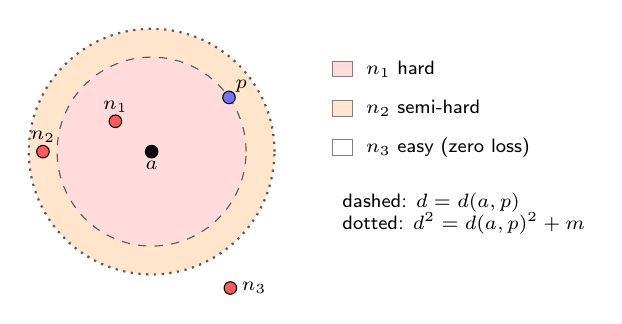
\begin{tikzpicture}[font=\sffamily\scriptsize, >=latex,
          pt/.style={circle, draw=black, inner sep=1.6pt},
          posp/.style={pt, fill=blue!55},
          negp/.style={pt, fill=red!65},
          ancp/.style={pt, fill=black}]
        % dashed radius d(a,p) = 1.2; dotted radius sqrt(1.2^2 + m) = 1.56
        \fill[orange!20] (0,0) circle (1.56);
        \fill[red!14] (0,0) circle (1.2);
        \draw[dashed, gray!70!black] (0,0) circle (1.2);
        \draw[dotted, thick, gray!70!black] (0,0) circle (1.56);
        \node[ancp] at (0,0) {};
        \node[anchor=north, inner sep=1pt] at (0,-0.08) {$a$};
        \node[posp] at (35:1.2) {};
        \node[anchor=south west, inner sep=1pt] at (35:1.25) {$p$};
        \node[negp] at (140:0.6) {};
        \node[anchor=south, inner sep=1pt, yshift=2pt] at (140:0.6) {$n_1$};
        \node[negp] at (180:1.38) {};
        \node[anchor=south, inner sep=1pt, yshift=2pt] at (180:1.38) {$n_2$};
        \node[negp] at (300:2.0) {};
        \node[anchor=west, inner sep=1pt, xshift=3pt] at (300:2.0) {$n_3$};
        \fill[red!14] (2.3,0.95) rectangle (2.55,1.15);
        \draw[gray] (2.3,0.95) rectangle (2.55,1.15);
        \node[anchor=west] at (2.6,1.05) {$n_1$ hard};
        \fill[orange!20] (2.3,0.45) rectangle (2.55,0.65);
        \draw[gray] (2.3,0.45) rectangle (2.55,0.65);
        \node[anchor=west] at (2.6,0.55) {$n_2$ semi-hard};
        \draw[gray] (2.3,-0.05) rectangle (2.55,0.15);
        \node[anchor=west] at (2.6,0.05) {$n_3$ easy (zero loss)};
        \node[anchor=north west, align=left] at (2.3,-0.4) {dashed: $d=d(a,p)$\\dotted: $d^2=d(a,p)^2+m$};
      \end{tikzpicture}}\\[0.3em]
      {\scriptsize Negatives seen from the anchor: closer than the positive (hard), inside the margin (semi-hard), or beyond it with zero loss (easy).\par}
      \vspace{0.5em}
      {\scriptsize Schroff et al., \href{https://arxiv.org/abs/1503.03832v3}{arXiv:1503.03832v3}, Sec.~3.2; Hermans et al., ``In Defense of the Triplet Loss for Person Re-Identification,'' arXiv 2017, \href{https://arxiv.org/abs/1703.07737v4}{arXiv:1703.07737v4}, Sec.~2, Eq.~5, Table~1.\par}
  \end{columns}
\end{frame}

\begin{frame}{Supervised Contrastive Learning (SupCon)}
  \begin{columns}[T,onlytextwidth]
    \column{0.52\textwidth}
      \begin{itemize}\footnotesize\itemsep0.22em
        \item NT-Xent gives each anchor one positive, its other augmented view. \textbf{SupCon} (Khosla et al., NeurIPS 2020) also treats every other batch image of the anchor's class as a positive:
        \[ \mathcal{L}^{\text{sup}}_{\text{out}}=\sum_{i\in I}\frac{-1}{|P(i)|}\sum_{p\in P(i)}\log\frac{\exp(z_i\cdot z_p/\tau)}{\sum_{a\in A(i)}\exp(z_i\cdot z_a/\tau)} \]
        $I$: the $2N$ augmented views of $N$ images; $A(i)=I\setminus\{i\}$; $P(i)\subseteq A(i)$: the views with the label of $i$; $z$: unit-norm projection-head output; $\tau$: temperature.
        \item \textbf{Where the average sits matters:} putting the sum over $P(i)$ and the $1/|P(i)|$ inside the log gives 67.4\% ImageNet top-1, against 78.7\% for the form above (ResNet-50, batch 6{,}144).
        \item Many positives and negatives per anchor weight hard examples through the gradient, so no explicit mining is needed.
        \item Two stages: SupCon trains the encoder, then a linear probe is fit on the frozen features.
      \end{itemize}
    \column{0.46\textwidth}
      \centering
      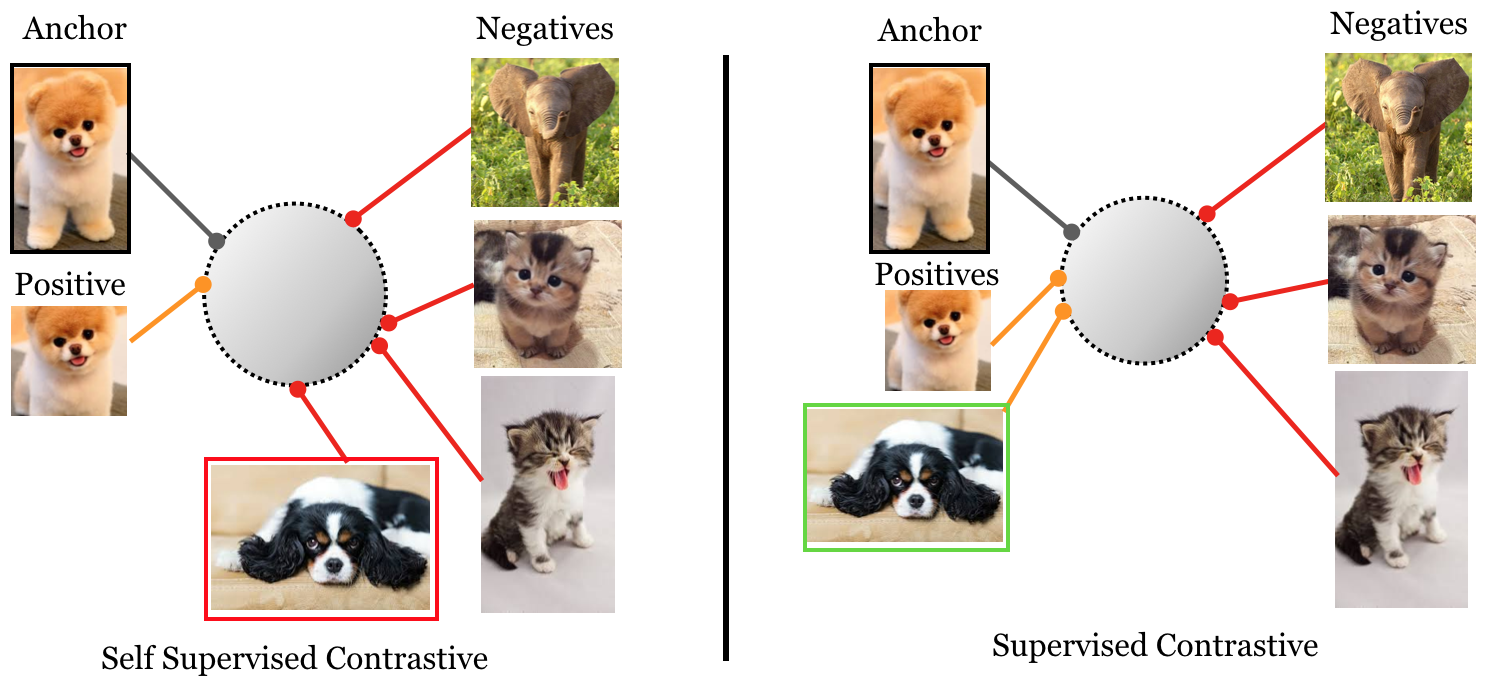
\includegraphics[width=\linewidth,height=0.40\textheight,keepaspectratio]{images/image-recognition/supcon_fig2_selfsup_vs_supervised_positives.png}\\[0.2em]
      {\scriptsize Khosla et al., ``Supervised Contrastive Learning,'' NeurIPS 2020, \href{https://arxiv.org/abs/2004.11362v5}{arXiv:2004.11362v5}, Figure~2; numbers from Sec.~3.2 and Tables~1 and~3.\par}
      \vspace{0.6em}
      {\scriptsize\setlength{\tabcolsep}{4pt}
      \begin{tabular}{@{}l c c@{}}
        \toprule
        \textbf{ImageNet top-1 (\%)} & \textbf{Cross-entropy} & \textbf{SupCon} \\
        \midrule
        ResNet-50 & 78.2 & 78.7 \\
        ResNet-200 & 80.9 & 81.4 \\
        \bottomrule
      \end{tabular}\par}
      \vspace{0.2em}
      {\scriptsize Same augmentation within each row (Table~3).\par}
  \end{columns}
\end{frame}

\begin{frame}{Proxies: One Learnable Point per Class}
  \begin{itemize}\footnotesize\itemsep0.3em
    \item \textbf{Proxy:} a learnable vector $p_c$ for each class $c$, trained with the network; each image is compared with the $C$ proxies instead of with other images. With $M$ training images an epoch costs $O(MC)$ comparisons, against $O(M^2)$ for pairs and $O(M^3)$ for triplets.
    \item \textbf{Proxy-NCA} (Movshovitz-Attias et al., ICCV 2017; NCA: neighbourhood components analysis):
    \[ \ell(x)=-\log\frac{e^{s(x,p^+)}}{\sum_{p^-\in P^-}e^{s(x,p^-)}} \]
    $s$: cosine similarity; $p^+$: the proxy of the class of $x$; $P^-$: the other proxies. It converged about three times as fast as triplet-based losses.
    \item \textbf{Proxy Anchor} (Kim et al., CVPR 2020) makes each proxy the anchor and compares it with every embedding in the batch:
    \[ \ell(X)=\frac{1}{|P^+|}\sum_{p\in P^+}\log\Big(1+\!\sum_{x\in X_p^+}\!e^{-\alpha(s(x,p)-\delta)}\Big)+\frac{1}{|P|}\sum_{p\in P}\log\Big(1+\!\sum_{x\in X_p^-}\!e^{\alpha(s(x,p)+\delta)}\Big) \]
    $X_p^+$ ($X_p^-$): batch embeddings of (not of) the class of $p$; $P^+$: proxies of the classes in the batch; $P$: all proxies; scale $\alpha=32$, margin $\delta=0.1$. The log-sum-exp gives harder examples larger gradients.
  \end{itemize}
  \vspace{0.2em}
  {\scriptsize Movshovitz-Attias et al., ``No Fuss Distance Metric Learning using Proxies,'' ICCV 2017, \href{https://arxiv.org/abs/1703.07464v3}{arXiv:1703.07464v3}; Kim et al., ``Proxy Anchor Loss for Deep Metric Learning,'' CVPR 2020, \href{https://arxiv.org/abs/2003.13911v1}{arXiv:2003.13911v1}, Eqs.~1 and~4.\par}
\end{frame}

\begin{frame}{ArcFace: An Additive Angular Margin}
  \begin{columns}[T,onlytextwidth]
    \column{0.56\textwidth}
      \begin{itemize}\footnotesize\itemsep0.3em
        \item \textbf{Classification as proxy learning:} drop the bias and normalise the class weights $W_j$ and the feature $x_i$; the logit becomes $\cos\theta_j$, and each $W_j$ acts as a proxy for class $j$ (Zhai and Wu, BMVC 2019). At test time $x_i$ is the embedding.
        \item \textbf{ArcFace} (Deng et al., CVPR 2019) adds a margin $m$ to the angle of the true class:
        \[ \mathcal{L}_{\text{Arc}}=-\frac{1}{N}\sum_{i=1}^{N}\log\frac{e^{s\cos(\theta_{y_i}+m)}}{e^{s\cos(\theta_{y_i}+m)}+\sum_{j\neq y_i}e^{s\cos\theta_j}} \]
        $N$: batch size; $y_i$: class of image $i$; $s$: a scale, since cosines in $[-1,1]$ cannot make the softmax confident. ArcFace used $s=64$, $m=0.5$, 512-d features.
        \item \textbf{Target logit:} normalised softmax $\cos\theta_y$; CosFace $\cos\theta_y-m$ (Wang et al., CVPR 2018); ArcFace $\cos(\theta_y+m)$, a margin in angle, i.e.\ geodesic distance on the sphere.
        \item No pair sampling: its authors name the ``combinatorial explosion'' of triplets as a drawback of the triplet loss.
      \end{itemize}
    \column{0.42\textwidth}
      \centering
      \vspace{0.4em}
      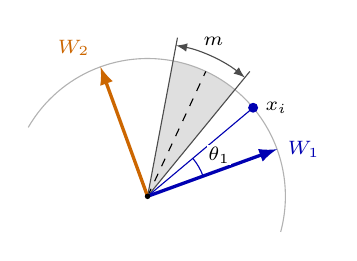
\begin{tikzpicture}[font=\sffamily\scriptsize, >=latex]
        % W1 at 20 deg, W2 at 110 deg, m = 0.5 rad = 28.65 deg. A point at angle phi between them goes to
        % class 1 when (phi-20)+m < 110-phi, i.e. phi < 50.68; to class 2 when phi > 79.32 (band width m).
        \fill[gray!25] (0,0) -- (50.68:1.75) arc[start angle=50.68, end angle=79.32, radius=1.75] -- cycle;
        \draw[gray!60] (-15:1.75) arc[start angle=-15, end angle=150, radius=1.75];
        \draw[dashed] (0,0) -- (65:1.75);
        \draw[gray!60!black] (0,0) -- (50.68:2.05);
        \draw[gray!60!black] (0,0) -- (79.32:2.05);
        \draw[<->, gray!60!black] (50.68:1.95) arc[start angle=50.68, end angle=79.32, radius=1.95];
        \node[anchor=south] at (65:1.98) {$m$};
        \draw[->, very thick, blue!70!black] (0,0) -- (20:1.75) node[anchor=west] {$W_1$};
        \draw[->, very thick, orange!80!black] (0,0) -- (110:1.75) node[anchor=south east] {$W_2$};
        \draw[blue!70!black] (0,0) -- (40:1.75);
        \fill[blue!70!black] (40:1.75) circle (1.8pt);
        \node[anchor=west, xshift=1pt] at (40:1.75) {$x_i$};
        \draw[blue!70!black] (20:0.75) arc[start angle=20, end angle=40, radius=0.75];
        \node[fill=white, inner sep=0.6pt] at (30:1.05) {$\theta_1$};
        \fill (0,0) circle (1pt);
      \end{tikzpicture}\\[0.3em]
      {\scriptsize Two classes on the unit circle during training. Dashed: the boundary without a margin (the bisector). ArcFace makes each class win by angle $m$, so the two boundaries open a band of width $m$ (grey).\par}
      \vspace{0.5em}
      {\scriptsize Deng et al., ``ArcFace: Additive Angular Margin Loss for Deep Face Recognition,'' CVPR 2019, \href{https://openaccess.thecvf.com/content_CVPR_2019/papers/Deng_ArcFace_Additive_Angular_Margin_Loss_for_Deep_Face_Recognition_CVPR_2019_paper.pdf}{OpenAccess}, Eq.~3; Zhai and Wu, ``Classification is a Strong Baseline for Deep Metric Learning,'' BMVC 2019, \href{https://arxiv.org/abs/1811.12649v2}{arXiv:1811.12649v2}; Wang et al., ``CosFace: Large Margin Cosine Loss for Deep Face Recognition,'' CVPR 2018, \href{https://arxiv.org/abs/1801.09414v2}{arXiv:1801.09414v2}.\par}
  \end{columns}
\end{frame}

\begin{frame}{A Metric Learning Reality Check}
  \begin{columns}[T,onlytextwidth]
    \column{0.55\textwidth}
      \begin{itemize}\footnotesize\itemsep0.4em
        \item Musgrave et al.\ (ECCV 2020) re-ran 13 losses from 2006--2019 under one protocol: BN-Inception (Inception with batch normalisation) pretrained on ImageNet, 128-d embeddings, batch 32, one augmentation recipe, hyperparameters from Bayesian optimisation with 4-fold cross-validation on the training classes, 10 runs per loss.
        \item \textbf{What papers had done:} changed backbone, embedding size or augmentation between compared methods; tuned on the test set; cited weak baselines, such as a triplet margin of 1 where about 0.1 works best.
        \item \textbf{Hidden details:} one paper's code froze the backbone's BatchNorm parameters, worth 2 points on CUB according to its authors, without saying so in the paper.
        \item \textbf{Finding:} newer losses ``perform marginally better than, and sometimes on par with, classic methods'' (table).
      \end{itemize}
    \column{0.43\textwidth}
      \centering
      \vspace{0.2em}
      {\scriptsize MAP@$R$ (\%), mean of 10 runs, 512-d (four 128-d models concatenated)\par}
      \vspace{0.3em}
      {\scriptsize\setlength{\tabcolsep}{4pt}
      \begin{tabular}{@{}l c c c@{}}
        \toprule
        \textbf{Loss (year)} & \textbf{CUB} & \textbf{Cars} & \textbf{SOP} \\
        \midrule
        No training (PCA to 512-d) & 14.21 & 5.91 & 23.44 \\
        Contrastive pair (2006) & 26.53 & 24.89 & 44.39 \\
        Triplet (2006) & 23.69 & 23.02 & 43.37 \\
        NT-Xent (2016) & 25.09 & 24.40 & 45.31 \\
        Proxy-NCA (2017) & 24.21 & 25.38 & 47.22 \\
        Norm.\ softmax (2017) & 25.25 & 26.00 & 47.13 \\
        CosFace (2018) & 26.70 & 27.57 & 46.92 \\
        ArcFace (2019) & 26.45 & 27.22 & 47.41 \\
        \bottomrule
      \end{tabular}\par}
      \vspace{0.4em}
      {\scriptsize Musgrave et al., \href{https://arxiv.org/abs/2003.08505v3}{arXiv:2003.08505v3}, Tables~4--7, Secs.~2--5.\par}
  \end{columns}
\end{frame}

\begin{frame}{Metric Learning Results After 2020}

  {\centering\scriptsize Recall@1 (\%) on the zero-shot splits, each paper's own protocol. ViT-S/16, ViT-B/16: small and base ViTs with $16\times16$ patches.\par}
  \vspace{0.2em}
  {\centering\scriptsize\setlength{\tabcolsep}{3.5pt}
  \begin{tabular}{@{}>{\raggedright\arraybackslash}p{2.4cm} >{\raggedright\arraybackslash}p{3.9cm} >{\raggedright\arraybackslash}p{3.3cm} c c c c@{}}
    \toprule
    \textbf{Method} & \textbf{Idea} & \textbf{Backbone, pretraining} & \textbf{Dim} & \textbf{CUB} & \textbf{Cars} & \textbf{SOP} \\
    \midrule
    Proxy Anchor (2020) & proxy loss & BN-Inception, ImageNet-1k & 512 & 68.4 & 86.1 & 79.1 \\
    No training & frozen features & ViT-S/16, ImageNet-21k & 384 & 83.1 & 47.8 & 62.1 \\
    Hyp-ViT (2022) & hyperbolic embeddings & ViT-S/16, ImageNet-21k & 384 & 85.6 & 86.5 & 85.9 \\
    Hyp-DINO (2022) & same, from DINO weights & ViT-S/16, DINO on ImageNet-1k & 384 & 80.9 & 89.2 & 85.1 \\
    RS@k (2022) & smoothed Recall@$k$ as the loss & ViT-B/16, ImageNet-21k & 512 & n/a & 89.5 & 88.0 \\
    Unicom (2023) & ArcFace on 1M pseudo-classes & ViT-B/16, LAION-400M & 768 & 88.8 & 97.7 & 88.8 \\
    \bottomrule
  \end{tabular}\par}
  \vspace{0.3em}
  \begin{itemize}\scriptsize\itemsep0.15em
    \item \textbf{Hyp-ViT:} embeddings in a Poincar\'e ball, a hyperbolic space whose volume grows exponentially with radius (suited to tree-like hierarchies), trained with an NT-Xent-style loss on hyperbolic distances. \textbf{RS@k} (Recall@$k$ surrogate): sigmoids replace the step functions that count ranks; batches of 4{,}000 images (392 on Cars196); SiMix mixes the similarities of same-class pairs. \textbf{Unicom}: CLIP features cluster LAION-400M into one million pseudo-classes.
    \item \textbf{On CUB, the pretraining data did most of the work:} frozen ImageNet-21k ViT-S features beat every CNN method in Ermolov et al.'s table on CUB (best 69.0); the authors suspect ImageNet-21k's bird classes. On Cars and SOP frozen features lag far behind, so training still matters.
  \end{itemize}
  \vspace{0.1em}
  {\scriptsize Kim et al., \href{https://arxiv.org/abs/2003.13911v1}{arXiv:2003.13911v1}, Tables~2--3; Ermolov et al., ``Hyperbolic Vision Transformers: Combining Improvements in Metric Learning,'' CVPR 2022, \href{https://arxiv.org/abs/2203.10833v2}{arXiv:2203.10833v2}, Table~3; Patel et al., ``Recall@k Surrogate Loss with Large Batches and Similarity Mixup,'' CVPR 2022, \href{https://arxiv.org/abs/2108.11179v2}{arXiv:2108.11179v2}, Table~2; An et al., ``Unicom: Universal and Compact Representation Learning for Image Retrieval,'' ICLR 2023, \href{https://arxiv.org/abs/2304.05884v1}{arXiv:2304.05884v1}, Tables~4 and~7.\par}
\end{frame}
